\subsection*{الف}
عملگر \text{\lr{Dilation}} با عنصر ساختاری قطری، معادل اجتماع تصویر با انتقال‌یافته‌های آن است:
\begin{flalign*}
SE_a &= {(-1,1), (0,0), (1,-1)} &&\
A \oplus SE_a &= \bigcup_{b \in SE_a} A_b = A_{(-1,1)} \cup A_{(0,0)} \cup A_{(1,-1)} &&
\end{flalign*}
\begin{center}
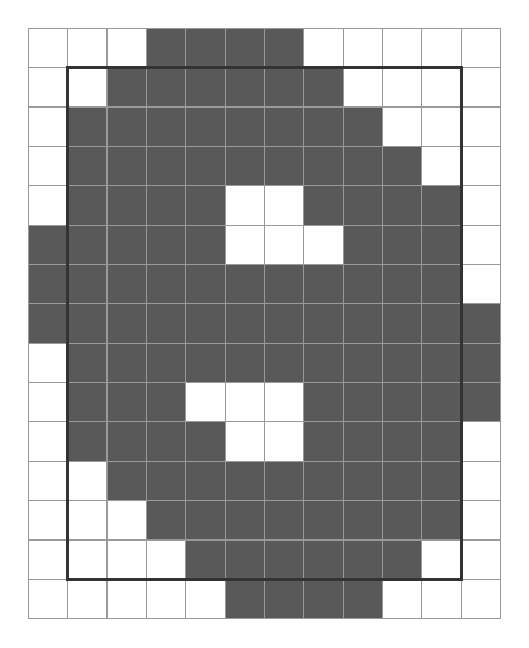
\begin{tikzpicture}[x=0.5cm, y=0.5cm]
\colorlet{gridcolor}{black!40}
\colorlet{fillcolor}{black!65}
\colorlet{origbox}{black!80}
\fill[fillcolor]
    (2,13) rectangle (6,14)
    (1,12) rectangle (7,13)
    (0,11) rectangle (8,12)
    (0,10) rectangle (9,11)
    (0,9)  rectangle (4,10)
    (6,9)  rectangle (10,10)
    (-1,8) rectangle (4,9)
    (7,8)  rectangle (10,9)
    (-1,7) rectangle (10,8)
    (-1,6) rectangle (11,7)
    (0,5)  rectangle (11,6)
    (0,4)  rectangle (3,5)
    (6,4)  rectangle (11,5)
    (0,3)  rectangle (4,4)
    (6,3)  rectangle (10,4)
    (1,2)  rectangle (10,3)
    (2,1)  rectangle (10,2)
    (3,0)  rectangle (9,1)
    (4,-1) rectangle (8,0);

\draw[step=1, gridcolor, thin] (-1,-1) grid (11,14);
\draw[origbox, very thick] (0,0) rectangle (10,13);
\end{tikzpicture}
\end{center}

\subsection*{ب}
عملگر \text{\lr{Erosion}} با عنصر ساختاری ستونی، تنها پیکسل‌هایی را حفظ می‌کند که همسایه‌های بالا و پایین آن‌ها در تصویر اصلی روشن باشند:
\begin{flalign*}
SE_b &= {(0,1), (0,0), (0,-1)} &&\
A \ominus SE_b &= {z \mid (SE_b)_z \subseteq A} &&
\end{flalign*}
\begin{center}
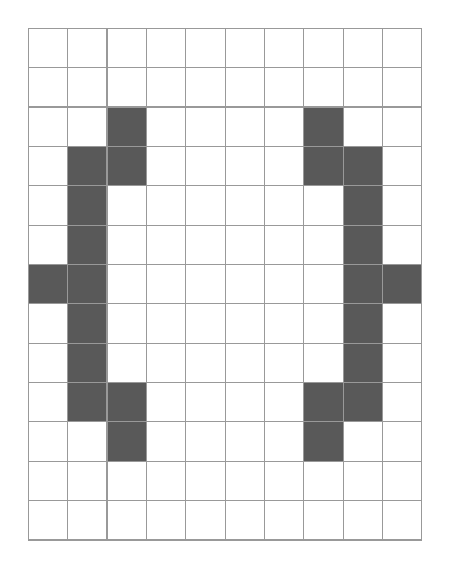
\begin{tikzpicture}[x=0.5cm, y=0.5cm]
\colorlet{gridcolor}{black!40}
\colorlet{fillcolor}{black!65}
\fill[fillcolor]
(2,9) rectangle (3,11)
(7,9) rectangle (8,11)
(1,3) rectangle (2,10)
(8,3) rectangle (9,10)
(2,2) rectangle (3,4)
(7,2) rectangle (8,4)
(0,6) rectangle (1,7)
(9,6) rectangle (10,7);
\draw[step=1, gridcolor, thin] (0,0) grid (10,13);
\end{tikzpicture}
\end{center}

\subsection*{ج}
عملگر \text{\lr{Opening}} معادل سایش و سپس بسط است و تنها بخش‌هایی از تصویر را حفظ می‌کند که عنصر ساختاری بتواند در آن‌ها محاط شود:
\begin{flalign*}
SE_c &= {(0,0), (-1,0), (1,0), (0,-1), (0,1)} &&\
A \circ SE_c &= (A \ominus SE_c) \oplus SE_c &&
\end{flalign*}
\begin{center}
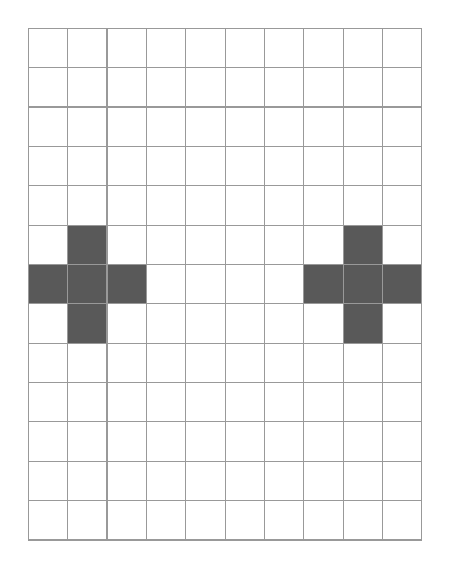
\begin{tikzpicture}[x=0.5cm, y=0.5cm]
\colorlet{gridcolor}{black!40}
\colorlet{fillcolor}{black!65}
\fill[fillcolor]
(1,5) rectangle (2,8)
(0,6) rectangle (3,7)
(8,5) rectangle (9,8)
(7,6) rectangle (10,7);
\draw[step=1, gridcolor, thin] (0,0) grid (10,13);
\end{tikzpicture}
\end{center}

\subsection*{د}
عملگر \text{\lr{Closing}} معادل بسط و سپس سایش است که باعث پر شدن گوشه‌های داخلی به اندازه عنصر ساختاری می‌شود:
\begin{flalign*}
SE_d &= {(0,0), (-1,0), (1,0), (0,-1), (0,1)} &&\
A \bullet SE_d &= (A \oplus SE_d) \ominus SE_d &&
\end{flalign*}
\begin{center}
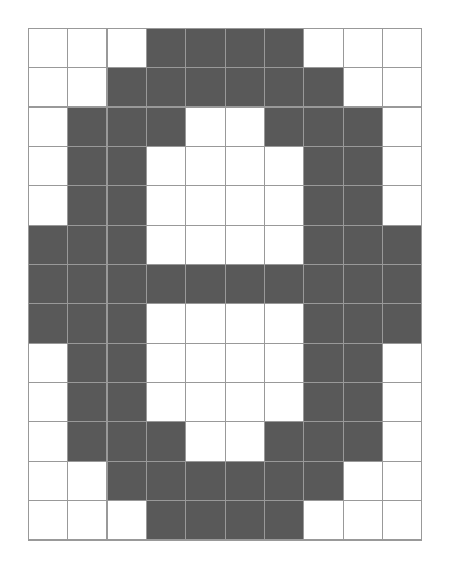
\begin{tikzpicture}[x=0.5cm, y=0.5cm]
\colorlet{gridcolor}{black!40}
\colorlet{fillcolor}{black!65}
\fill[fillcolor]
(3,12) rectangle (7,13)
(2,11) rectangle (8,12)
(1,10) rectangle (4,11)
(6,10) rectangle (9,11)
(1,8)  rectangle (3,10)
(7,8)  rectangle (9,10)
(0,7)  rectangle (3,8)
(7,7)  rectangle (10,8)
(0,6)  rectangle (10,7)
(0,5)  rectangle (3,6)
(7,5)  rectangle (10,6)
(1,3)  rectangle (3,5)
(7,3)  rectangle (9,5)
(1,2)  rectangle (4,3)
(6,2)  rectangle (9,3)
(2,1)  rectangle (8,2)
(3,0)  rectangle (7,1);
\draw[step=1, gridcolor, thin] (0,0) grid (10,13);
\end{tikzpicture}
\end{center}